\documentclass[a4paper,12pt]{article}

\usepackage{rotating}
\usepackage[top=1in, bottom=1in, left=0.75in, right=0.75in]{geometry}
\usepackage{graphicx}
\usepackage[numbers,square,sort&compress]{natbib}
\usepackage{setspace}
\usepackage[cdot,mediumqspace,]{SIunits}
\usepackage{caption}
\usepackage{subcaption}
\usepackage{mathtools}
\usepackage{authblk}
\usepackage{float}
\renewcommand{\thesubsection}{\thesection.\alph{subsection}}
\providecommand{\e}[1]{\ensuremath{\times 10^{#1}}}

\begin{document}
\onehalfspacing
\title{PHY 407 Lab 2}
\author{Natalie Price-Jones, 999091021}
\date{19 September 2014}
\affil{\small{natalie.price.jones@mail.utoronto.ca}}
\maketitle

\section{Question 1}
\subsection{Part b)}

\begin{figure}[H]
\centering
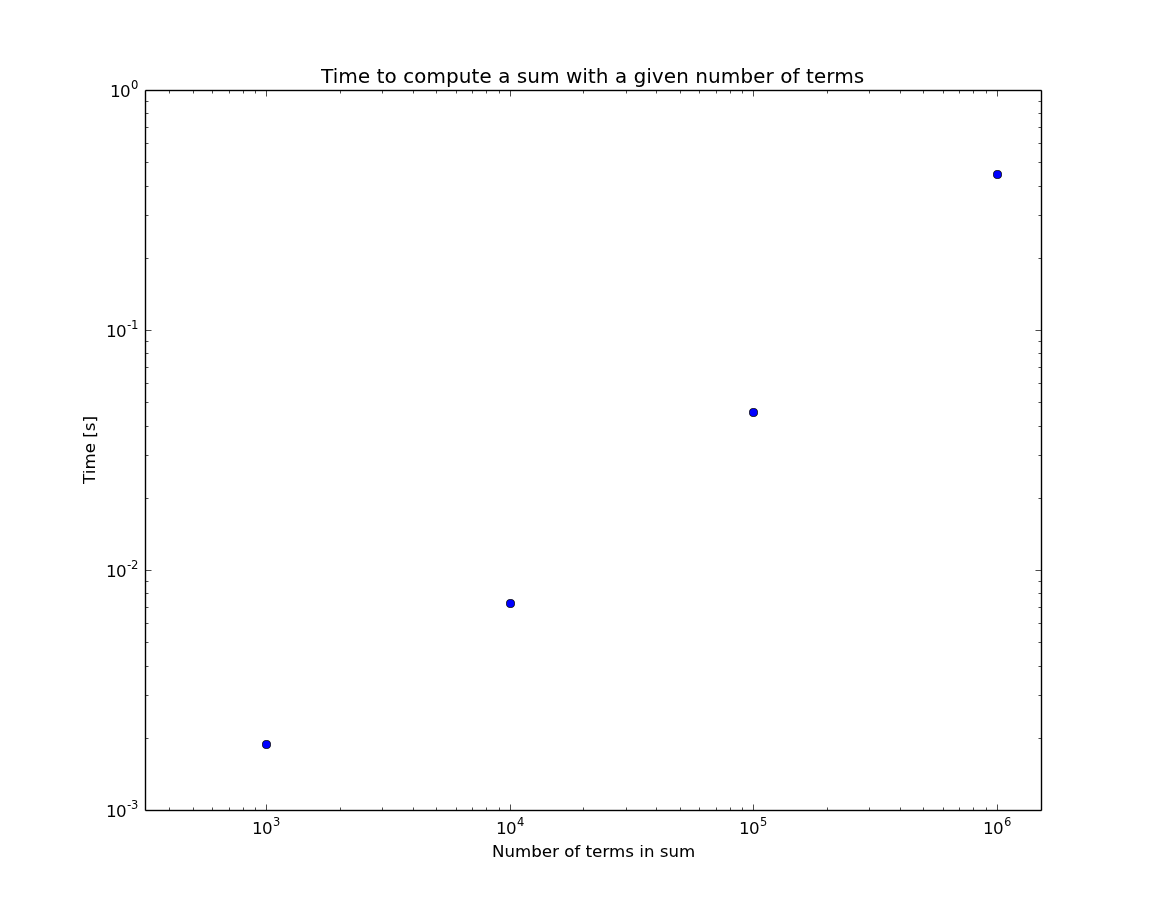
\includegraphics[width = \linewidth]{lab2q1b.png}
\caption{Time needed to compute a sum with a set number of terms. Both axes have been logscaled.}
\label{fig:q1}
\end{figure}

\subsection{Part c)}
The for loop that cycles through each term in the sum is given below:
\begin{verbatim}

[1] for n in range(terms):
[2]    E = n + 0.5
[3]    weight = exp(-beta*E)
[4]    S += weight*E
[5]    Z += weight

\end{verbatim}

We can explicitly count the number of floating point operations (flops) for each iteration of this loop. On line [2], we have 1 flop (addition). On line [3], there are 3 flops (two multiplications and an exponential). On line [4], there are 2 flops (addition and multiplication). On line [5], there is 1 flop (addition). Therefore our total tally is 7 flops per iteration of the loop.

\subsection{Part d)}

We can calculate the number of flops per second by first taking the number of terms in the sum, multiplied by the number of flops per iteration (i.e. per term). This gives the total of number of flops for each sum. Then we divide this total by the time it took to compute the sum.

\begin{equation}
flop/s = (flop/term)*(nterms)/time\nonumber
\end{equation}

In order to compare this to the June 2014 top supercomputer, we then divided this flop/s by the number of cores in my laptop (two cores). The value varied, depending on the number of terms in the sum, but the averages over 10 repetitions of the program averaged to around $1\e{6.74}$ flop/s/core (Figure \ref{fig:q1} had an average value of $1\e{6.7452}$ flop/s/core).

The top supercomputer for June 2014 according to www.top500.org could calculate $1\e{10}$ flop/s/core. This separates it from my laptop by about three and half orders of magnitude in speed.

\section{Question 2}
\subsection{Part b)}

The result of running the Python file called lab2\_q2.py is 4.40042666667. This is the calculated value of the integral of $x^4 - 2x + 1$ from 0 to 2 by dividing it into $N=10$ slices and approximating it with Simpson's Rule.

We can calculate the fractional error ($\epsilon$) in this result ($I_{calc}$) by comparing it with the known true result ($I_{true} = 4.4$).

\begin{eqnarray}
\epsilon &=& (I_{calc}-I_{true})/I_{true}\nonumber\\
\epsilon &=& (4.40042666667-4.4)/4.4\nonumber\\
\epsilon &=& 9.70\e{-5}\nonumber
\end{eqnarray}

So the fractional error in the result when the integral is approximated with Simpson's Rule is $9.70\e{-5}$

\subsection{Part c)}

\begin{table}[!htbp]
  \centering
  \begin{tabular}{|c||c||c||c||c|}
  \hline
   Number of Slices & Trapezoidal Rule & Fractional Error & Simpson's Rule & Fractional Error\\
   \hline
   \hline
   10 & 4.50656 & 2.4\e{-2} & 4.40042666667 & 9.7\e{-5}\\
   \hline
   100 & 4.401066656 & 2.4\e{-4} & 4.40000004267 & 9.7\e{-9}\\
   \hline
   1000 & 4.40001066667 & 2.4\e{-6} & 4.4 & 9.7\e{-13}\\
   \hline
   \end{tabular}
    \caption{Fractional errors for trapezoidal rule and Simpson's rule for increasing number of divisions in the region of interest. Fractional error represents the deviation from the true value of 4.4.}
    \label{tab:integrals}
\end{table}

It's easy to see that for the same number of slices, Simpson's rule gives vastly more accurate results.

\section{Question 3}

It is possible to calculate the error in an integral approximated with the trapezoidal rule with the following equation.

\begin{equation}
\epsilon = \frac{1}{3}|I_2-I_1|
\label{eqn:err}
\end{equation}

In Equation \ref{eqn:err}, $\epsilon$ is the error and $I_2$ is the evaluation of the integral with double the number of slices of those used to evaluate $I_1$. For the integral approximated with the trapezoid rule for $N = 10$ then $N = 20$ slices in the file lab2\_q3.py, this equation yields $\epsilon = 0.026633333333333137$. However, the actual deviation from the true value, $|I_2 - 4.4| = 0.026660000000000572$ does not match the estimation of the error given by Equation \ref{eqn:err}. This is because Equation \ref{eqn:err} is an approximation of the error. It quite obviously gives the right order of magnitude, but fails to represent precisely the error involved in the integral approximation.

\section{Question 4}

\subsection{Part c)}

\begin{figure}[H]
\centering
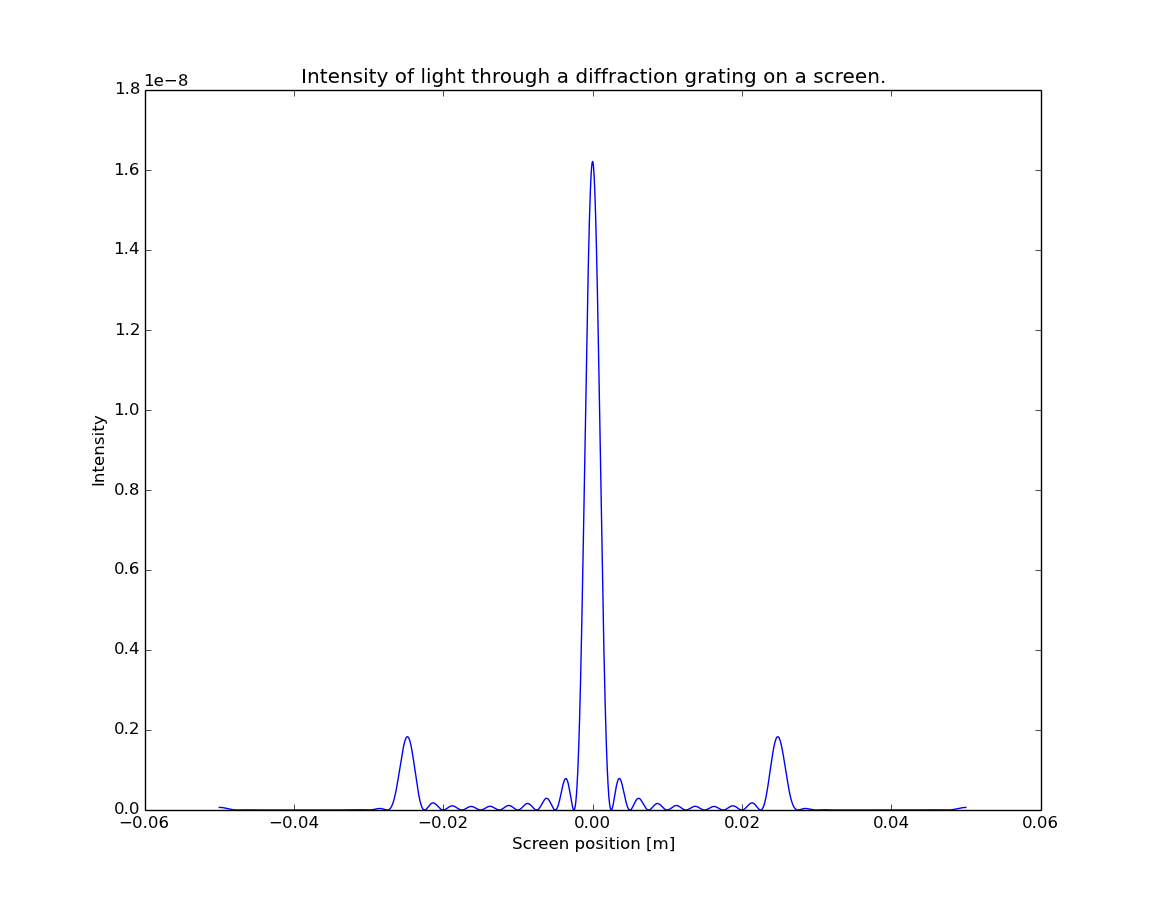
\includegraphics[width = \linewidth]{lab2q4c.png}
\caption{Intensity of light across a screen in one dimension for a transmission function given by $q(u) = sin^2(\alpha u)$.}
\label{fig:q4c}
\end{figure}

\subsection{Part d)}

\begin{figure}[H]
\centering

\includegraphics[width = \linewidth]{lab2q4d.png}
\caption{Intensity of light across a screen in two dimensions for a transmission function given by $q(u) = sin^2(\alpha u)$.}
\label{fig:q4d}
\end{figure}

\subsection{Part e)}
\subsubsection{Part i)}

\begin{figure}[H]
\centering

\includegraphics[width = \linewidth]{lab2q4ei.png}
\caption{Intensity of light across a screen in two dimensions for a transmission function given by $q(u) = sin^2(\alpha u) sin^2(\beta u)$.}
\label{fig:q4ei}
\end{figure}

\subsubsection{Part ii)}

\begin{figure}[H]
\centering

\includegraphics[width = \linewidth]{lab2q4eii.png}
\caption{Intensity of light across a screen in two dimensions for a transmission function for square slits, one 10$\mu$m slit 60$\mu$m from a 20$\mu$m slit.}
\label{fig:q4eii}
\end{figure}

\end{document}